% This is "sig-alternate.tex" V2.0 May 2012
% This file should be compiled with V2.5 of "sig-alternate.cls" May 2012
%
% This example file demonstrates the use of the 'sig-alternate.cls'
% V2.5 LaTeX2e document class file. It is for those submitting
% articles to ACM Conference Proceedings WHO DO NOT WISH TO
% STRICTLY ADHERE TO THE SIGS (PUBS-BOARD-ENDORSED) STYLE.
% The 'sig-alternate.cls' file will produce a similar-looking,
% albeit, 'tighter' paper resulting in, invariably, fewer pages.
%
% ----------------------------------------------------------------------------------------------------------------
% This .tex file (and associated .cls V2.5) produces:
%       1) The Permission Statement
%       2) The Conference (location) Info information
%       3) The Copyright Line with ACM data
%       4) NO page numbers
%
% as against the acm_proc_article-sp.cls file which
% DOES NOT produce 1) thru' 3) above.
%
% Using 'sig-alternate.cls' you have control, however, from within
% the source .tex file, over both the CopyrightYear
% (defaulted to 200X) and the ACM Copyright Data
% (defaulted to X-XXXXX-XX-X/XX/XX).
% e.g.
% \CopyrightYear{2007} will cause 2007 to appear in the copyright line.
% \crdata{0-12345-67-8/90/12} will cause 0-12345-67-8/90/12 to appear in the copyright line.
%
% ---------------------------------------------------------------------------------------------------------------
% This .tex source is an example which *does* use
% the .bib file (from which the .bbl file % is produced).
% REMEMBER HOWEVER: After having produced the .bbl file,
% and prior to final submission, you *NEED* to 'insert'
% your .bbl file into your source .tex file so as to provide
% ONE 'self-contained' source file.
%
% ================= IF YOU HAVE QUESTIONS =======================
% Questions regarding the SIGS styles, SIGS policies and
% procedures, Conferences etc. should be sent to
% Adrienne Griscti (griscti@acm.org)
%
% Technical questions _only_ to
% Gerald Murray (murray@hq.acm.org)
% ===============================================================
%
% For tracking purposes - this is V2.0 - May 2012

\documentclass{sig-alternate-05-2015}
\usepackage{epstopdf}
\usepackage{pgfplots}
\usepgfplotslibrary{external}


\begin{document}
%
% --- Author Metadata here ---
%\conferenceinfo{WOODSTOCK}{'97 El Paso, Texas USA}
%\CopyrightYear{2007} % Allows default copyright year (20XX) to be over-ridden - IF NEED BE.
%\crdata{0-12345-67-8/90/01}  % Allows default copyright data (0-89791-88-6/97/05) to be over-ridden - IF NEED BE.
% --- End of Author Metadata ---

\title{Proposed Method of Information Retrieval and Display from the US Federal Register}
%\subtitle{[Extended Abstract]}
%
% You need the command \numberofauthors to handle the 'placement
% and alignment' of the authors beneath the title.
%
% For aesthetic reasons, we recommend 'three authors at a time'
% i.e. three 'name/affiliation blocks' be placed beneath the title.
%
% NOTE: You are NOT restricted in how many 'rows' of
% "name/affiliations" may appear. We just ask that you restrict
% the number of 'columns' to three.
%
% Because of the available 'opening page real-estate'
% we ask you to refrain from putting more than six authors
% (two rows with three columns) beneath the article title.
% More than six makes the first-page appear very cluttered indeed.
%
% Use the \alignauthor commands to handle the names
% and affiliations for an 'aesthetic maximum' of six authors.
% Add names, affiliations, addresses for
% the seventh etc. author(s) as the argument for the
% \additionalauthors command.
% These 'additional authors' will be output/set for you
% without further effort on your part as the last section in
% the body of your article BEFORE References or any Appendices.

\numberofauthors{3} %  in this sample file, there are a *total*
% of EIGHT authors. SIX appear on the 'first-page' (for formatting
% reasons) and the remaining two appear in the \additionalauthors section.
%
\author{
% You can go ahead and credit any number of authors here,
% e.g. one 'row of three' or two rows (consisting of one row of three
% and a second row of one, two or three).
%
% The command \alignauthor (no curly braces needed) should
% precede each author name, affiliation/snail-mail address and
% e-mail address. Additionally, tag each line of
% affiliation/address with \affaddr, and tag the
% e-mail address with \email.
%
% 1st. author
\alignauthor
Matthew J Wiecek\\
       \affaddr{Texas A\&M University}\\
       \affaddr{College Station, TX}\\
       \email{matthewwiecek@tamu.edu}
% 2nd. author
\alignauthor
Chun-Chan (Bill) Cheng\\
        \affaddr{Texas A\&M University}\\
       \affaddr{College Station, TX}\\
       \email{aznchat@tamu.edu}
% 3rd. author
\alignauthor
Divyesh M Tekale\\
        \affaddr{Texas A\&M University}\\
       \affaddr{College Station, TX}\\
       \email{tekale2@tamu.edu}
}
\setcopyright{rightsretained}
% There's nothing stopping you putting the seventh, eighth, etc.
% author on the opening page (as the 'third row') but we ask,
% for aesthetic reasons that you place these 'additional authors'
% in the \additional authors block, viz.
% Just remember to make sure that the TOTAL number of authors
% is the number that will appear on the first page PLUS the
% number that will appear in the \additionalauthors section.

\maketitle
\begin{abstract}
The US Federal Government posts many Notices, Proposed Rules, Final Rules, Presidential Documents, and other documents of consequence on a daily basis. Being able to search and navigate through all of these documents in a rapid fashion is of the utmost importance in many legal and political fields. We propose a system that will graph the search results in a hierarchical structure to clearly indicate which federal agency published the document. We further propose that the results be color-coded to easily identify the type of document retrieved. 
\end{abstract}

\begin{CCSXML}
<ccs2012>
<concept>
<concept_id>10002951.10003317.10003359.10011699</concept_id>
<concept_desc>Information systems~Presentation of retrieval results</concept_desc>
<concept_significance>500</concept_significance>
</concept>
<concept>
<concept_id>10002951.10003317.10003371.10003381.10003382</concept_id>
<concept_desc>Information systems~Structured text search</concept_desc>
<concept_significance>300</concept_significance>
</concept>
<concept>
<concept_id>10002951.10003317.10003371.10010852.10003393</concept_id>
<concept_desc>Information systems~Enterprise search</concept_desc>
<concept_significance>300</concept_significance>
</concept>
</ccs2012>
\end{CCSXML}

\ccsdesc[500]{Information systems~Presentation of retrieval results}
\ccsdesc[300]{Information systems~Structured text search}
\ccsdesc[300]{Information systems~Enterprise search}
\printccsdesc

\terms{Theory}

\keywords{Federal Register, Graph Output, Information Retrieval}

\section{Introduction}
The US Federal Register is the official Daily Journal of the United States government. All Federal Notices, Proposed Rules, Final Rules, Presidential Documents, et cetera, are published by the Register. Any document published in the Register carries legal significance as they are considered to constitute legal notice to the public. Being able to rapidly search through the Federal Register and interpret the results is a valuable ability for any legal counsel. 

In particular, the layout of the search results is crucial. Upon presentation, the user should immediately be able to identify the type of document as well as the the publishing agency. Owing to the hierarchical structure of government, a graph structure can quickly represent which agency published a document and where it lies in the federal bureaucracy. A color coding scheme may be used to denote the type of document presented.

\section{High Level Overview of System}
\subsection{Subsystems}
The system shall be made up of three distinct subsystems: the crawler, the search engine, and the user interface. The crawler will interact with the Federal Register API to fetch the documents and process them into a format that is acceptable to the search engine. The search engine shall serve user queries and return a list of documents that match the query. The user interface shall be responsible for handling user interaction and displaying the search results returned by the search engine.

\subsubsection{Crawler and the Federal Register API}
The Federal Register maintains an API to allow developers access to federal documents.\footnote{The documentation to the API may be found at https://www.federalregister.gov/learn/developers} As the API has a limit of 1000 documents per request, the crawler shall request the full set of each day's documents one day at a time. It is not expected that there shall be more than 1000 documents published by the Federal Government on any given day. The response shall be parsed and returned to the search engine for indexing. 

\subsubsection{Search Engine and Apache Solr}
The search engine used will be Apache Solr. 

\subsubsection{User Interface and the Web Browser}
Users will interact with the search engine via a web interface. The user will be free to input a query via a text box. There will be further filtering options available, such as restricting the search to certain federal departments or agencies. The user query will then be passed to the search engine via an HTML GET request. Upon receipt of the response from the search engine, the web page will be responsible for drawing the graph and color coding the elements. 

\subsection{Timeline of Events}
There are two events during the application's life. The initial launch of the application, and a user query.

\subsubsection{Launch of Application}
Upon launch of the application, both Solr and the Web Crawler will launch (see Figure 1). Due to the 1000 item limit per API call imposed by the Federal Register API, the crawler will request documents one day at a time. Once the documents have been fetched and processed, the crawler shall forward the crawled documents to Solr for indexing. The crawler will the update its own internal record of which days have already been crawled, and begin crawling the earliest day that has not yet been crawled. This will continue indefinitely until program termination or an error encounter within the crawler.

\subsubsection{User Query}
Once the user enters the query, pre-processing occurs, including any trimming and possible spelling correction. The query is then forwarded via an HTTP GET request to Solr for fulfillment. Solr will return a list of potential documents that match the result with associated meta-data. The web page will render the results and display any spelling recommendations that have been executed. At this point the user will be free to interact with the search results, such as expanding them to get the abstract, or a link to the document itself.

\begin{figure}
\centering
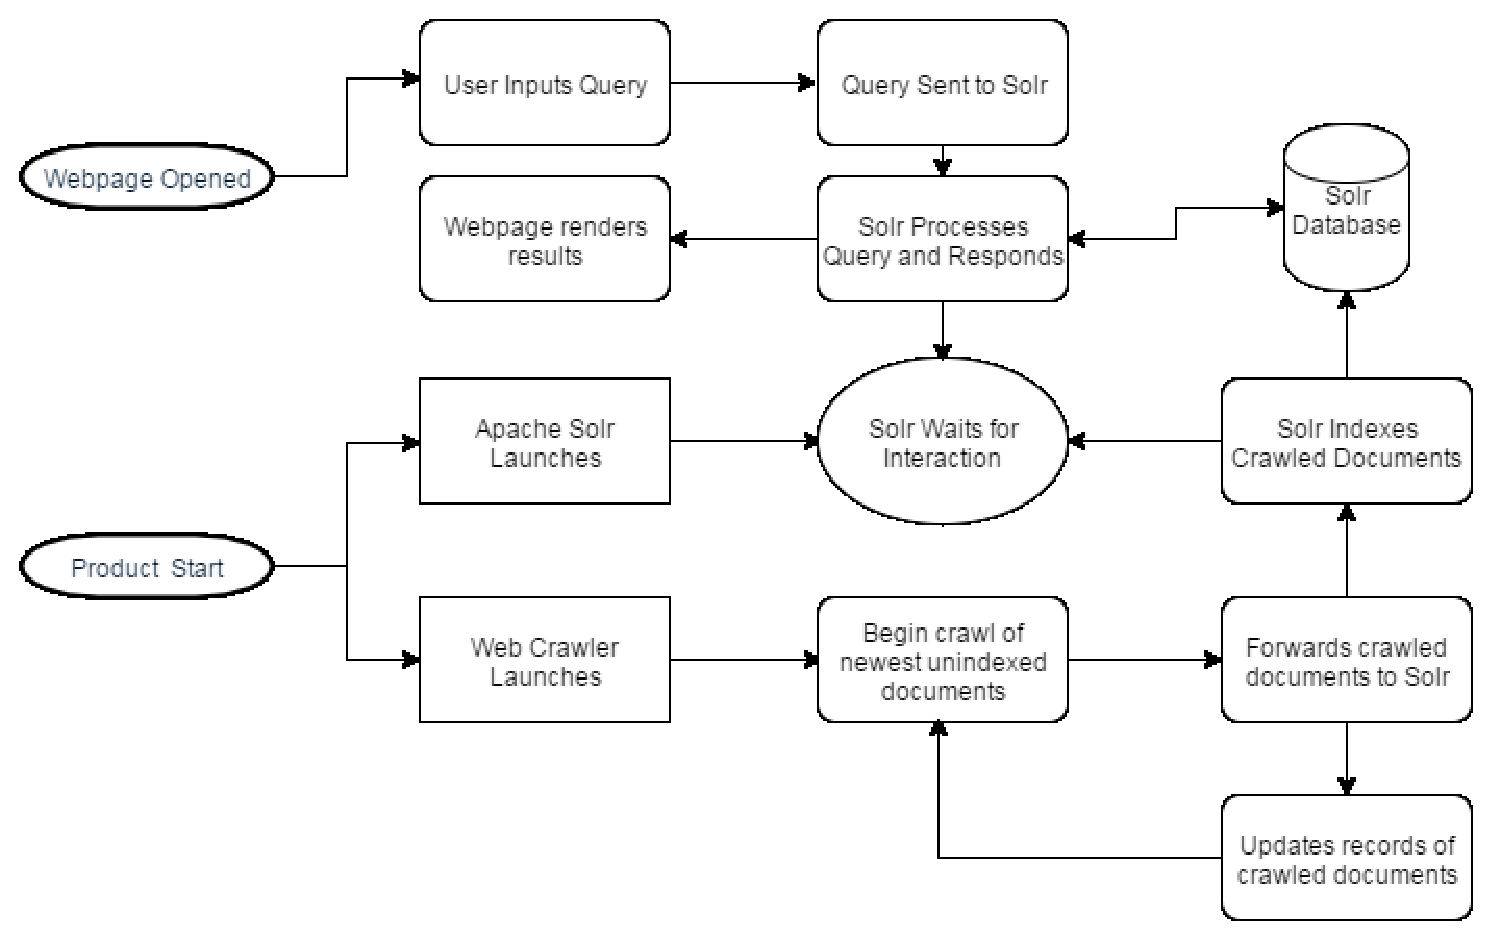
\epsfig{file=Solr_Workflow.eps, width = 240pt}
\caption{The sequence of events in the application}
\end{figure}

\section{Low Level Overview of Subsystems}
\subsection{Web Crawler \& Federal Register API}
The webcrawler will be written in \emph{Java} and will be composed of several individual subsystems. 
\subsubsection{Query Generation}
The Federal Register maintains an API that is accessible via standard HTTP GET requests. The request has been crafted to request a JSON object containing the links to the XML versions of each published document. As the API sets a maximum limit of 1000 items per request, a query will be generated to request each day's published documents; the assumption is that there will never be more than 1000 unique documents published in any given day. The class \emph{Generate\_Queries} is responsible for generating the web requests. It implements the runnable interface, allowing other threads to run as it generates the queries. The generated query is then pushed into a \emph{BlockingQueue} which is thread-safe so that other threads may execute the queries.

\subsubsection{Fetching \& Parsing JSON Response}
Once the queries have been generated, an HTTP request has to be served over the network to retrieve the JSON object from the Federal Register API that contains the links to the XML versions of that days documents. This is the responsibility of \emph{Get\_List\_Docs}. It fetches the queries from a \emph{BlockingQueue}, sends the GET request, and parses the JSON response. The extracted URLS are put into a different \emph{BlockingQueue} so that other threads may fetch the documents themselves. This class also implements the runnable interface to parallelize the fetching of the JSON responses. As there is no interaction necessary between different \emph{Get\_List\_Docs}, many threads can be spawned to ensure that the network is saturated.

\subsubsection{Retrieval of Published Documents}
Once the URL of the XML version of the document has been retreived, the actual document must be retrieved over the network. The class \emph{Get\_Doc} retrieves the actual document itself. It, also, implements the runnable interface. The number of threads can be increased to ensure that the network is saturated. It fetches the URL to the XML version of the document from a \emph{BlockingQueue}. After fetching the document, this thread will be responsible for any necessary parsing of the document before being handed off to the Search Engine for indexing.

\subsubsection{Network Abstraction}
Network requests take some management, such as opening a socket and handling relevant error codes. As such, a class \emph{Network}, abstracts away such considerations and presents a simple interface for performing GET requests. It simply contains \emph{static} methods which can be executed by other functions. 

\section{Statistics on the Getting the Documents}
The following figure is the statistics we ran on different number of threads to fetch the data from the webpage.\\


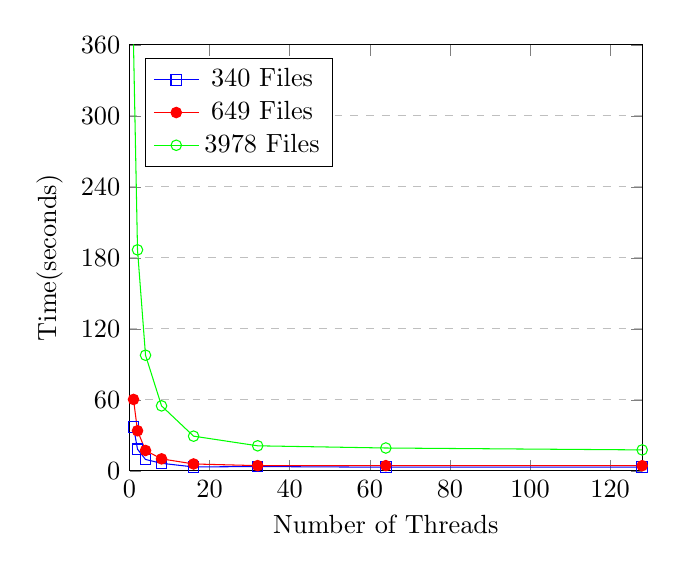
\begin{tikzpicture}[scale=0.95]
\begin{axis}[
    xlabel={Number of Threads},
    ylabel={Time(seconds)},
    xmin=0, xmax=128,
    ymin=0, ymax=360,
    xtick={0,20,40,60,80,100,120},
    ytick={0,60,120,180,240,300,360},
    legend pos=north west,
    ymajorgrids=true,
    grid style=dashed,
]
\legend{340 Files,649 Files, 3978 Files}

\addplot[color=blue, mark=square,]
    coordinates {
    (1,37.110)(2,18.229)(4,9.589)(8,6.331)(16,3.275)(32,3.597)(64,3.032)(128,3.160)
    };
  
\addplot[color=red, mark=*, ]
    coordinates {
    (1,60.337)(2,33.860)(4,17.175)(8,10.096)(16,5.785)(32,4.375)(64,4.359)(128,4.309)
    };
\addplot[color=green, mark=o, ]
    coordinates {
    (1,360.459)(2,186.753)(4,97.714)(8,54.892)(16,29.284)(32,21.127)(64,19.270)(128,17.667)
    }; 
\end{axis}
\end{tikzpicture}

As you can see in the figure, we have three lines indicating different numbers of data we crawled with the x-axis as the number of thread and y-axis as the system time. In the figure it can be seen that there is a limit in increasing the threads to increase the speed of fetching the webpages. In fact, the slope gradually slows down when the thread numbers gets to 32. In conclusion, we fetched 1400 days (11000 documents) in less than three minutes with 100 threads running.  



%\subsection{References} %Uncomment if we add references

%
% The below is commented out, remove at some point
%
\if false

\section{Below is From Template, REMOVE}
\subsection{Citations}
Citations to articles \cite{bowman:reasoning,
clark:pct, braams:babel, herlihy:methodology},
conference proceedings \cite{clark:pct} or
books \cite{salas:calculus, Lamport:LaTeX} listed
in the Bibliography section of your
article will occur throughout the text of your article.
You should use BibTeX to automatically produce this bibliography;
you simply need to insert one of several citation commands with
a key of the item cited in the proper location in
the \texttt{.tex} file \cite{Lamport:LaTeX}.
The key is a short reference you invent to uniquely
identify each work; in this sample document, the key is
the first author's surname and a
word from the title.  This identifying key is included
with each item in the \texttt{.bib} file for your article.

The details of the construction of the \texttt{.bib} file
are beyond the scope of this sample document, but more
information can be found in the \textit{Author's Guide},
and exhaustive details in the \textit{\LaTeX\ User's
Guide}\cite{Lamport:LaTeX}.

This article shows only the plainest form
of the citation command, using \texttt{{\char'134}cite}.
This is what is stipulated in the SIGS style specifications.
No other citation format is endorsed or supported.

\subsection{Tables}
Because tables cannot be split across pages, the best
placement for them is typically the top of the page
nearest their initial cite.  To
ensure this proper ``floating'' placement of tables, use the
environment \textbf{table} to enclose the table's contents and
the table caption.  The contents of the table itself must go
in the \textbf{tabular} environment, to
be aligned properly in rows and columns, with the desired
horizontal and vertical rules.  Again, detailed instructions
on \textbf{tabular} material
is found in the \textit{\LaTeX\ User's Guide}.

Immediately following this sentence is the point at which
Table 1 is included in the input file; compare the
placement of the table here with the table in the printed
dvi output of this document.

\begin{table}
\centering
\caption{Frequency of Special Characters}
\begin{tabular}{|c|c|l|} \hline
Non-English or Math&Frequency&Comments\\ \hline
\O & 1 in 1,000& For Swedish names\\ \hline
$\pi$ & 1 in 5& Common in math\\ \hline
\$ & 4 in 5 & Used in business\\ \hline
$\Psi^2_1$ & 1 in 40,000& Unexplained usage\\
\hline\end{tabular}
\end{table}

To set a wider table, which takes up the whole width of
the page's live area, use the environment
\textbf{table*} to enclose the table's contents and
the table caption.  As with a single-column table, this wide
table will ``float" to a location deemed more desirable.
Immediately following this sentence is the point at which
Table 2 is included in the input file; again, it is
instructive to compare the placement of the
table here with the table in the printed dvi
output of this document.


\begin{table*}
\centering
\caption{Some Typical Commands}
\begin{tabular}{|c|c|l|} \hline
Command&A Number&Comments\\ \hline
\texttt{{\char'134}alignauthor} & 100& Author alignment\\ \hline
\texttt{{\char'134}numberofauthors}& 200& Author enumeration\\ \hline
\texttt{{\char'134}table}& 300 & For tables\\ \hline
\texttt{{\char'134}table*}& 400& For wider tables\\ \hline\end{tabular}
\end{table*}
% end the environment with {table*}, NOTE not {table}!

\subsection{Figures}
Like tables, figures cannot be split across pages; the
best placement for them
is typically the top or the bottom of the page nearest
their initial cite.  To ensure this proper ``floating'' placement
of figures, use the environment
\textbf{figure} to enclose the figure and its caption.

This sample document contains examples of \textbf{.eps}
and \textbf{.ps} files to be displayable with \LaTeX.  More
details on each of these is found in the \textit{Author's Guide}.

\begin{figure}
\centering
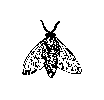
\epsfig{file=fly.eps}
\caption{A sample black and white graphic (.eps format).}
\end{figure}

\begin{figure}
\centering
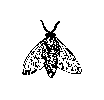
\epsfig{file=fly.eps, height=1in, width=1in}
\caption{A sample black and white graphic (.eps format)
that has been resized with the \texttt{epsfig} command.}
\end{figure}


As was the case with tables, you may want a figure
that spans two columns.  To do this, and still to
ensure proper ``floating'' placement of tables, use the environment
\textbf{figure*} to enclose the figure and its caption.
and don't forget to end the environment with
{figure*}, not {figure}!

\begin{figure*}
\centering
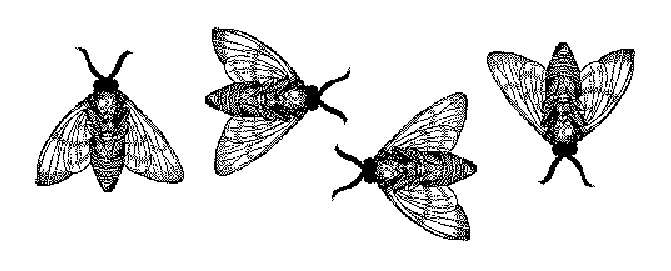
\epsfig{file=flies.eps}
\caption{A sample black and white graphic (.eps format)
that needs to span two columns of text.}
\end{figure*}

Note that either {\textbf{.ps}} or {\textbf{.eps}} formats are
used; use
the \texttt{{\char'134}epsfig} or \texttt{{\char'134}psfig}
commands as appropriate for the different file types.


\subsection{Theorem-like Constructs}
Other common constructs that may occur in your article are
the forms for logical constructs like theorems, axioms,
corollaries and proofs.  There are
two forms, one produced by the
command \texttt{{\char'134}newtheorem} and the
other by the command \texttt{{\char'134}newdef}; perhaps
the clearest and easiest way to distinguish them is
to compare the two in the output of this sample document:

This uses the \textbf{theorem} environment, created by
the\linebreak\texttt{{\char'134}newtheorem} command:
\newtheorem{theorem}{Theorem}
\begin{theorem}
Let $f$ be continuous on $[a,b]$.  If $G$ is
an antiderivative for $f$ on $[a,b]$, then
\begin{displaymath}\int^b_af(t)dt = G(b) - G(a).\end{displaymath}
\end{theorem}

The other uses the \textbf{definition} environment, created
by the \texttt{{\char'134}newdef} command:
\newdef{definition}{Definition}
\begin{definition}
If $z$ is irrational, then by $e^z$ we mean the
unique number which has
logarithm $z$: \begin{displaymath}{\log e^z = z}\end{displaymath}
\end{definition}

Two lists of constructs that use one of these
forms is given in the
\textit{Author's  Guidelines}.
 
There is one other similar construct environment, which is
already set up
for you; i.e. you must \textit{not} use
a \texttt{{\char'134}newdef} command to
create it: the \textbf{proof} environment.  Here
is a example of its use:
\begin{proof}
Suppose on the contrary there exists a real number $L$ such that
\begin{displaymath}
\lim_{x\rightarrow\infty} \frac{f(x)}{g(x)} = L.
\end{displaymath}
Then
\begin{displaymath}
l=\lim_{x\rightarrow c} f(x)
= \lim_{x\rightarrow c}
\left[ g{x} \cdot \frac{f(x)}{g(x)} \right ]
= \lim_{x\rightarrow c} g(x) \cdot \lim_{x\rightarrow c}
\frac{f(x)}{g(x)} = 0\cdot L = 0,
\end{displaymath}
which contradicts our assumption that $l\neq 0$.
\end{proof}

Complete rules about using these environments and using the
two different creation commands are in the
\textit{Author's Guide}; please consult it for more
detailed instructions.  If you need to use another construct,
not listed therein, which you want to have the same
formatting as the Theorem
or the Definition\cite{salas:calculus} shown above,
use the \texttt{{\char'134}newtheorem} or the
\texttt{{\char'134}newdef} command,
respectively, to create it.

\subsection*{A {\secit Caveat} for the \TeX\ Expert}
Because you have just been given permission to
use the \texttt{{\char'134}newdef} command to create a
new form, you might think you can
use \TeX's \texttt{{\char'134}def} to create a
new command: \textit{Please refrain from doing this!}
Remember that your \LaTeX\ source code is primarily intended
to create camera-ready copy, but may be converted
to other forms -- e.g. HTML. If you inadvertently omit
some or all of the \texttt{{\char'134}def}s recompilation will
be, to say the least, problematic.

\section{Conclusions}
This paragraph will end the body of this sample document.
Remember that you might still have Acknowledgments or
Appendices; brief samples of these
follow.  There is still the Bibliography to deal with; and
we will make a disclaimer about that here: with the exception
of the reference to the \LaTeX\ book, the citations in
this paper are to articles which have nothing to
do with the present subject and are used as
examples only.
%\end{document}  % This is where a 'short' article might terminate

%ACKNOWLEDGMENTS are optional
\section{Acknowledgments}
This section is optional; it is a location for you
to acknowledge grants, funding, editing assistance and
what have you.  In the present case, for example, the
authors would like to thank Gerald Murray of ACM for
his help in codifying this \textit{Author's Guide}
and the \textbf{.cls} and \textbf{.tex} files that it describes.

%
% The following two commands are all you need in the
% initial runs of your .tex file to
% produce the bibliography for the citations in your paper.
\bibliographystyle{abbrv}
\bibliography{sigproc}  % sigproc.bib is the name of the Bibliography in this case
% You must have a proper ".bib" file
%  and remember to run:
% latex bibtex latex latex
% to resolve all references
%
% ACM needs 'a single self-contained file'!
%
%APPENDICES are optional
%\balancecolumns
\appendix
%Appendix A
\section{Headings in Appendices}
The rules about hierarchical headings discussed above for
the body of the article are different in the appendices.
In the \textbf{appendix} environment, the command
\textbf{section} is used to
indicate the start of each Appendix, with alphabetic order
designation (i.e. the first is A, the second B, etc.) and
a title (if you include one).  So, if you need
hierarchical structure
\textit{within} an Appendix, start with \textbf{subsection} as the
highest level. Here is an outline of the body of this
document in Appendix-appropriate form:
\subsection{Introduction}
\subsection{The Body of the Paper}
\subsubsection{Type Changes and  Special Characters}
\subsubsection{Math Equations}
\paragraph{Inline (In-text) Equations}
\paragraph{Display Equations}
\subsubsection{Citations}
\subsubsection{Tables}
\subsubsection{Figures}
\subsubsection{Theorem-like Constructs}
\subsubsection*{A Caveat for the \TeX\ Expert}
\subsection{Conclusions}
\subsection{Acknowledgments}
\texttt{{\char'134}additionalauthors} command at the start
of the document.

Generated by bibtex from your ~.bib file.  Run latex,
then bibtex, then latex twice (to resolve references)
to create the ~.bbl file.  Insert that ~.bbl file into
the .tex source file and comment out
the command \texttt{{\char'134}thebibliography}.
% This next section command marks the start of
% Appendix B, and does not continue the present hierarchy
\section{More Help for the Hardy}
The sig-alternate.cls file itself is chock-full of succinct
and helpful comments.  If you consider yourself a moderately
experienced to expert user of \LaTeX, you may find reading
it useful but please remember not to change it.
%\balancecolumns % GM June 2007
% That's all folks!

\fi
%
%
%

\end{document}
